% ============================================================
%  Progetto di Esame — Elementi di Intelligenza Artificiale
%  Ottimizzazione Automatica dell'Architettura di Reti Neurali
%  tramite Algoritmo Genetico
% ============================================================

\documentclass[12pt, a4paper]{article}

% ── Encoding e lingua ────────────────────────────────────────
\usepackage[utf8]{inputenc}
\usepackage[T1]{fontenc}
\usepackage[italian]{babel}

% ── Layout pagina ────────────────────────────────────────────
\usepackage[top=2.5cm, bottom=2.5cm, left=3cm, right=3cm]{geometry}

% ── Tipografia ───────────────────────────────────────────────
\usepackage{lmodern}
\usepackage{microtype}
\usepackage{setspace}
\onehalfspacing

% ── Matematica ───────────────────────────────────────────────
\usepackage{amsmath}
\usepackage{amssymb}

% ── Codice sorgente ──────────────────────────────────────────
\usepackage{listings}
\usepackage{xcolor}

\definecolor{codebg}{RGB}{245,245,245}
\definecolor{codeblue}{RGB}{46,64,87}
\definecolor{codegray}{RGB}{120,120,120}
\definecolor{codegreen}{RGB}{40,120,40}

\lstset{
    backgroundcolor=\color{codebg},
    basicstyle=\ttfamily\small,
    keywordstyle=\color{codeblue}\bfseries,
    commentstyle=\color{codegreen}\itshape,
    stringstyle=\color{orange!80!black},
    language=Python,
    breaklines=true,
    frame=single,
    rulecolor=\color{gray!40},
    numbers=left,
    numberstyle=\tiny\color{codegray},
    numbersep=8pt,
    tabsize=4,
    showstringspaces=false,
    captionpos=b,
    xleftmargin=15pt
}

% ── Tabelle ──────────────────────────────────────────────────
\usepackage{booktabs}
\usepackage{array}
\usepackage{colortbl}
\usepackage{multirow}
\definecolor{headerblue}{RGB}{46,117,182}
\definecolor{rowgray}{RGB}{242,242,242}

% ── Immagini ─────────────────────────────────────────────────
\usepackage{graphicx}
\usepackage{float}
\usepackage{caption}
\usepackage{subcaption}

% ── Riquadri e note ──────────────────────────────────────────
\usepackage{tcolorbox}
\tcbuselibrary{skins}

% riquadro per le domande frequenti / concetti chiave
\newtcolorbox{concetto}[1]{
    colback=blue!5!white,
    colframe=blue!50!black,
    fonttitle=\bfseries,
    title=#1,
    rounded corners,
    left=6pt, right=6pt, top=4pt, bottom=4pt
}

% riquadro per le domande che potrebbero fare la prof
\newtcolorbox{domanda}{
    colback=orange!8!white,
    colframe=orange!70!black,
    fonttitle=\bfseries,
    title={Possibile domanda d'esame},
    rounded corners,
    left=6pt, right=6pt, top=4pt, bottom=4pt
}

% riquadro attenzione
\newtcolorbox{attenzione}{
    colback=red!5!white,
    colframe=red!60!black,
    fonttitle=\bfseries,
    title={Attenzione},
    rounded corners,
    left=6pt, right=6pt, top=4pt, bottom=4pt
}

% ── Link ─────────────────────────────────────────────────────
\usepackage{hyperref}
\hypersetup{
    colorlinks=true,
    linkcolor=blue!60!black,
    urlcolor=blue!60!black,
    pdftitle={Progetto IA — Neural Architecture Search tramite GA},
}

% ── Intestazioni ─────────────────────────────────────────────
\usepackage{fancyhdr}
\pagestyle{fancy}
\fancyhf{}
\fancyhead[L]{\small\textit{Neural Architecture Search tramite Algoritmo Genetico}}
\fancyhead[R]{\small\thepage}
\renewcommand{\headrulewidth}{0.4pt}

% ── Titolo ───────────────────────────────────────────────────
\title{
    \vspace{-1cm}
    {\Large Progetto di Esame — Elementi di Intelligenza Artificiale}\\[0.8cm]
    {\huge \textbf{Ottimizzazione Automatica}}\\[0.3cm]
    {\huge \textbf{dell'Architettura di Reti Neurali}}\\[0.3cm]
    {\huge \textbf{tramite Algoritmo Genetico}}\\[1cm]
    {\large Corso di Laurea Triennale in Ingegneria Informatica}
}
\author{}
\date{\today}

% ════════════════════════════════════════════════════════════
\begin{document}
% ════════════════════════════════════════════════════════════

\maketitle
\thispagestyle{empty}
\vspace{1cm}

\begin{abstract}
Questo documento descrive il progetto realizzato per l'esame di Elementi di
Intelligenza Artificiale. Il sistema implementato combina una rete neurale
costruita da zero in Python con un Algoritmo Genetico (GA) per automatizzare
la ricerca della migliore architettura della rete sul dataset Iris.
L'approccio rientra nel campo della Neural Architecture Search (NAS) e
dimostra come due paradigmi di ottimizzazione --- il calcolo del gradiente e
l'evoluzione biologica --- possano collaborare per risolvere un problema di
classificazione multi-classe.
\end{abstract}

\newpage
\tableofcontents
\newpage

% ════════════════════════════════════════════════════════════
\section{Introduzione}
% ════════════════════════════════════════════════════════════

Il progetto affronta il problema della \textbf{Neural Architecture Search (NAS)},
ovvero la ricerca automatica della migliore architettura di una rete neurale
per un dato problema. Tradizionalmente, la progettazione di una rete neurale
richiede che il ricercatore scelga manualmente il numero di layer, il numero
di neuroni per layer e le funzioni di attivazione. Questa scelta è spesso
guidata dall'esperienza e da tentativi ed errori, rendendo il processo lungo
e dipendente dall'expertise del progettista.

L'obiettivo di questo progetto è automatizzare questa scelta utilizzando un
\textbf{Algoritmo Genetico}, che esplora lo spazio delle possibili architetture e
converge verso quelle che massimizzano l'accuratezza sul dataset Iris, tenendo
conto anche della complessità computazionale della rete tramite una funzione
di penalità.

\subsection{NAS}

Il NAS è la tecnica per automatizzare la progettazione di reti neurali artificiali (ANN) ovvero un modello ampiamente utilizzato nel machine learning. Serve come detto per evitare la specifica manuale dell'architettura di una rete neurale la quale potrebbe non essere ottimale in termini di efficienza e complessità spaziale e temporale.

NAS è strettamente correlato all'ottimizzazione degli iperparametri e al meta-apprendimento ed è un sottocampo dell'\textit{automated machine learning}.

\begin{itemize}
    \item Gli \textbf{iperparametri} sono parametri che possono essere impostati per definire qualsiasi parte configurabile del processo di apprendimento di un modello
    
    Sono ad esempio:

    \begin{itemize}
        \item learning rate
        \item topologia della rete
        \item dimensione della rete
        \item etc
    \end{itemize}
    
    \item Il \textbf{meta learning} o \textbf{meta-apprendimento}, definito anche "apprendere ad apprendere", è una sottocategoria del machine learning che addestra i modelli di intelligenza artificiale (AI) a comprendere e ad adattarsi autonomamente alle nuove attività. L'obiettivo principale del meta learning è quello di fornire alle macchine le competenze necessarie per apprendere ad apprendere.
    
    Ciò che abbiamo implementato è un caso di \textbf{ottimizzazione annidata}: il GA opera a un livello superiore ottimizzando la struttura, mentre la backpropagation opera a un livello inferiore ottimizzando i pesi. C'è quindi una gerarchia di due ottimizzatori che agiscono su scale e parametri diversi.

    Questo si avvicina concettualmente al meta-apprendimento, ma se ne differenzia nella sostanza: il meta-apprendimento vero accumula esperienza su molti dataset per estrarre principi generali di apprendimento. Il nostro sistema è specifico per un singolo dataset, quindi è più corretto definirlo \textit{architecture search} che meta-learning.

    Ad esempio, un vero sistema di meta-learning imparerebbe: "i problemi con feature continue e poche classi tendono a beneficiare di reti con ReLU e pochi layer" --- principio valido su dataset diversi, non solo su Iris.
\end{itemize}




\subsection{Originalità e Rilevanza Pratica}

Il progetto non è originale nel senso accademico del termine --- la NAS esiste
dagli anni '90. Tuttavia il suo contributo è dimostrare la comprensione
profonda di due paradigmi fondamentali dell'AI e la capacità di farli
interagire. Il filone di ricerca esplorato è oggi uno dei più attivi nel campo:
modelli come \textit{EfficientNet} di Google nascono da processi automatici di
ricerca dell'architettura, e la NAS è ampiamente usata in contesti industriali
dove si deve deployare una rete su hardware con risorse limitate.

\begin{domanda}
\textit{``Il tuo progetto è originale?''}\\
No, nel senso accademico stretto. La NAS tramite GA è una tecnica nota. Ciò
che è originale è la combinazione specifica: una rete neurale scritta da zero
con backpropagation implementata manualmente, integrata con un GA che ne
ottimizza l'architettura, con penalità di complessità e valutazione multipla
(K=3) per ridurre la varianza. Tutti i componenti sono costruiti senza
librerie di machine learning preconfezionate.
\end{domanda}

\newpage

% ════════════════════════════════════════════════════════════
\section{Background Teorico}
% ════════════════════════════════════════════════════════════

% ────────────────────────────────────────────────────────────
\subsection{Reti Neurali Artificiali}
% ────────────────────────────────────────────────────────────

Una rete neurale artificiale è un modello computazionale ispirato al
funzionamento del cervello biologico. È composta da unità elementari
chiamate \textbf{neuroni}, organizzati in layer successivi. Ogni neurone riceve
input dal layer precedente, li combina linearmente tramite pesi e bias,
e applica una funzione di attivazione non lineare per produrre il proprio output.

\subsubsection{Struttura di un Neurone e dei Layer}

Per un singolo neurone $i$ l'output è:
\begin{equation}
    a_i = f\!\left(\mathbf{w}_i^T \mathbf{x} + b_i\right)
\end{equation}
Raggruppando tutti i neuroni di un layer in forma matriciale:
\begin{equation}
    \mathbf{a} = f\!\left(\mathbf{W}\mathbf{x} + \mathbf{b}\right)
\end{equation}

dove $\mathbf{W}$ è la matrice dei pesi, $\mathbf{x}$ il vettore di input,
$\mathbf{b}$ il vettore dei bias e $f$ la funzione di attivazione.

La struttura di una rete feed-forward è composta da tre tipologie di layer:

\begin{itemize}
    \item \textbf{Layer di input} --- riceve le feature del dataset senza
          applicare nessuna trasformazione.
    \item \textbf{Hidden layer} --- trasforma la rappresentazione dei dati
          applicando combinazioni lineari seguite da funzioni di attivazione
          non lineari.
    \item \textbf{Layer di output} --- produce la predizione finale con una
          funzione di attivazione appropriata al tipo di problema.
\end{itemize}

\subsubsection{Funzioni di Attivazione}

Le funzioni di attivazione introducono la non linearità nella rete. Senza di
esse, layer multipli sarebbero equivalenti a un singolo layer lineare ---
indipendentemente dalla profondità, la rete potrebbe solo rappresentare
trasformazioni lineari dell'input, incapace di apprendere pattern complessi.

\vspace{0.3cm}
\noindent\textbf{ReLU (Rectified Linear Unit)}
\begin{equation}
    f(x) = \max(0, x), \qquad f'(x) = \begin{cases} 1 & x > 0 \\ 0 & x \leq 0 \end{cases}
\end{equation}
È la funzione più usata negli hidden layer perché computazionalmente
efficiente e \emph{mitiga} il problema del vanishing gradient per
valori positivi: la sua derivata è esattamente 1, quindi il contributo
della funzione di attivazione al gradiente non si riduce attraversando
il layer (a differenza di Sigmoid che satura). Ha però il problema
dei \textit{neuroni morti}: se il valore di pre-attivazione
$z = \mathbf{w}^T\mathbf{x} + b$ di un neurone è sistematicamente
negativo, ReLU restituisce sempre 0 e la derivata è sempre 0.
Il neurone smette di ricevere aggiornamenti e non impara più nulla.
Leaky ReLU nasce proprio per risolvere questo limite.

\vspace{0.3cm}
\noindent\textbf{Leaky ReLU}
\begin{equation}
    f(x) = \max(0.01x,\; x), \qquad f'(x) = \begin{cases} 1 & x > 0 \\ 0.01 & x \leq 0 \end{cases}
\end{equation}
Variante di ReLU che risolve il problema dei neuroni morti permettendo un
piccolo gradiente anche per valori negativi.

\vspace{0.3cm}
\noindent\textbf{Sigmoid}
\begin{equation}
    f(x) = \frac{1}{1+e^{-x}}, \qquad f'(x) = f(x)\bigl(1-f(x)\bigr)
\end{equation}
Comprime l'output nell'intervallo $(0,1)$. Soffre del problema del gradiente
che svanisce per valori molto grandi o molto piccoli (\textit{vanishing gradient}).

\vspace{0.3cm}
\noindent\textbf{Softmax}
\begin{equation}
    f(x_i) = \frac{e^{x_i}}{\displaystyle\sum_j e^{x_j}}
\end{equation}
Trasforma un vettore di valori arbitrari in una distribuzione di probabilità
(tutti i valori tra 0 e 1, somma = 1). È la funzione ideale per il layer di
output in problemi di \textbf{classificazione multi-classe} come Iris.

\begin{concetto}{Perché Softmax solo sull'output layer?}
La Softmax è definita su un vettore e il suo output dipende da \emph{tutti}
i valori del vettore contemporaneamente. Applicarla in un hidden layer
creerebbe due problemi: (1) tutti i neuroni del layer dovrebbero sommare a 1,
forzandoli a \emph{competere} tra loro invece di apprendere feature
indipendenti; (2) se il layer avesse un solo neurone, l'operazione
$e^{x}/e^{x} = 1$ darebbe costantemente 1, azzerando il gradiente e
bloccando l'apprendimento. Negli hidden layer si usano funzioni
elemento-per-elemento come ReLU e Sigmoid.
\end{concetto}

\begin{domanda}
\textit{``Perché usi l'approssimazione diagonale della derivata della Softmax?''}\\
La derivata completa della Softmax è una matrice --- il Jacobiano --- perché
ogni output dipende da tutti gli input. L'elemento $(i,j)$ del Jacobiano è:
\[
    \frac{\partial f_i}{\partial x_j} =
    \begin{cases} f_i(1-f_i) & i=j \\ -f_i f_j & i \neq j \end{cases}
\]
Nell'implementazione si usa solo la diagonale $f_i(1-f_i)$, che coincide con
la formula della Sigmoid. Questa approssimazione evita di dover modificare
la struttura della backpropagation (che si aspetta vettori, non matrici) ed
è sufficiente perché su Iris le classi sono ben separabili e la rete
converge comunque correttamente.
\end{domanda}

% ────────────────────────────────────────────────────────────
\subsubsection{Backpropagation}
% ────────────────────────────────────────────────────────────

La backpropagation è l'algoritmo standard per addestrare reti neurali tramite
discesa del gradiente. Funziona in due fasi.

\vspace{0.2cm}
\noindent\textbf{Forward pass} --- l'input viene propagato attraverso tutti
i layer fino all'output. I valori intermedi (pre-attivazione $\mathbf{z}$ e
post-attivazione $\mathbf{a}$) vengono salvati perché necessari nella fase
successiva.

\vspace{0.2cm}
\noindent\textbf{Backward pass} --- l'errore viene propagato all'indietro
calcolando il gradiente della funzione di loss rispetto a ogni peso tramite
la \textbf{regola della catena}:
\begin{equation}
    \frac{\partial \mathcal{L}}{\partial \mathbf{W}^{(l)}} =
    \boldsymbol{\delta}^{(l)} \cdot \left(\mathbf{a}^{(l-1)}\right)^T
\end{equation}
dove $\boldsymbol{\delta}^{(l)}$ è il vettore dei delta del layer $l$.

\vspace{0.2cm}
La funzione di loss usata è il \textbf{Mean Squared Error (MSE)}:
\begin{equation}
    \mathcal{L} = \frac{1}{2}\sum_i \left(\hat{y}_i - y_i\right)^2,
    \qquad
    \frac{\partial \mathcal{L}}{\partial \hat{y}_i} = \hat{y}_i - y_i
\end{equation}

I pesi vengono aggiornati sottraendo il gradiente moltiplicato per il
learning rate $\eta$:
\begin{equation}
    \mathbf{W} \leftarrow \mathbf{W} - \eta \cdot \frac{\partial \mathcal{L}}{\partial \mathbf{W}}
\end{equation}

\begin{concetto}{Perché salvare i valori intermedi?}
L'implementazione mantiene \texttt{valori\_intermedi} e \texttt{valori\_input}
come attributi della rete perché il calcolo dei delta nella fase backward
richiede i valori pre-attivazione $\mathbf{z}^{(l)}$ (per applicare $f'$) e
le attivazioni $\mathbf{a}^{(l-1)}$ (per calcolare il gradiente dei pesi).
Senza salvarli durante il forward pass bisognerebbe ricalcolarli, raddoppiando
il costo computazionale.
\end{concetto}

% ────────────────────────────────────────────────────────────
\subsection{Algoritmi Genetici}
% ────────────────────────────────────────────────────────────

Gli algoritmi genetici sono metodi di ottimizzazione ispirati alla teoria
dell'evoluzione naturale di Darwin. Operano su una \textbf{popolazione} di
soluzioni candidate e le fanno evolvere attraverso generazioni successive
applicando operatori biologicamente ispirati.

\subsubsection{Concetti Fondamentali}

\begin{itemize}
    \item \textbf{Cromosoma} --- rappresentazione di una soluzione candidata.
          Nel progetto è una lista di tuple che descrive l'architettura della rete.
    \item \textbf{Gene} --- elemento atomico del cromosoma. Nel progetto ogni
          gene è una tupla \texttt{(n\_neuroni, funzione\_attivazione)}.
    \item \textbf{Fitness} --- misura della qualità di ogni individuo.
          Nel progetto è l'accuratezza sul validation set penalizzata per la complessità.
    \item \textbf{Generazione} --- un'iterazione completa del ciclo evolutivo.
    \item \textbf{Popolazione} --- l'insieme di tutti gli individui in una generazione.
\end{itemize}

\subsubsection{Il Ciclo Evolutivo}

\begin{enumerate}
    \item Generazione casuale della popolazione iniziale
    \item Valutazione della fitness di ogni individuo
    \item Selezione dei genitori (torneo)
    \item Generazione dei figli tramite crossover
    \item Mutazione dei figli
    \item Sostituzione della vecchia popolazione con la nuova
    \item Ripeti dal passo 2 per $N$ generazioni
\end{enumerate}

\subsubsection{Selezione Tramite Torneo}

La \textbf{selezione a torneo} bilancia due esigenze opposte che un buon GA
deve avere contemporaneamente:

\begin{itemize}
    \item \textbf{Sfruttamento} (\textit{exploitation}) --- i migliori individui
          devono avere più probabilità di riprodursi.
    \item \textbf{Esplorazione} (\textit{exploration}) --- anche individui
          mediocri devono avere qualche possibilità, per mantenere diversità
          genetica e ridurre il rischio di convergenza prematura verso ottimi locali.
\end{itemize}

\begin{domanda}
\textit{``Perché usi la selezione a torneo invece di selezionare sempre i migliori?''}\\
Se si selezionassero sempre i migliori, dopo poche generazioni tutta la
popolazione diventerebbe molto simile. Il GA smette di esplorare e converge
prematuramente su un ottimo locale. Con il torneo, estraiamo $k=3$ individui
a caso e scegliamo il migliore tra loro: un individuo forte ha alta probabilità
di vincere, ma uno mediocre ha ancora chance se gli capita un torneo con
avversari più deboli. La dimensione $k$ controlla il bilanciamento:
$k$ grande $\Rightarrow$ più pressione selettiva, $k$ piccolo $\Rightarrow$ più esplorazione.
\end{domanda}

% ────────────────────────────────────────────────────────────
\subsection{Neural Architecture Search}
% ────────────────────────────────────────────────────────────

La NAS è il campo di ricerca che studia come automatizzare la progettazione
di architetture di reti neurali. Questo progetto ne implementa una versione
semplificata: un GA che esplora lo spazio delle architetture usando come
funzione di fitness l'accuratezza ottenuta dopo training con backpropagation.

Il concetto chiave è la \textbf{separazione tra due livelli di ottimizzazione}:

\begin{itemize}
    \item Il \textbf{GA} ottimizza l'architettura --- parametri \emph{discreti}
          come numero di layer, neuroni e funzioni di attivazione. Non esiste
          un gradiente per questi parametri, quindi la discesa del gradiente
          non è applicabile.
    \item La \textbf{backpropagation} ottimizza i pesi all'interno di ogni
          architettura --- parametri \emph{continui}. Opera su scale temporali
          diverse e con un meccanismo completamente diverso.
\end{itemize}

\begin{domanda}
\textit{``Il tuo progetto usa il Reinforcement Learning?''}\\
No. Il RL è un paradigma in cui un agente impara agendo in un ambiente e
ricevendo reward. Il progetto usa un GA (ottimizzazione evolutiva) combinato
con backpropagation (ottimizzazione per gradiente). I modelli generativi come
le GAN o gli LLM sono anch'essi un campo separato. Il punto di contatto con
il RL esiste solo in alcune applicazioni avanzate (es. RLHF per LLM) che non
riguardano questo progetto.
\end{domanda}

\newpage

% ════════════════════════════════════════════════════════════
\section{Implementazione}
% ════════════════════════════════════════════════════════════

% ────────────────────────────────────────────────────────────
\subsection{Struttura del Progetto}
% ────────────────────────────────────────────────────────────

\begin{itemize}
    \item \texttt{nn\_layer.py} --- classe \texttt{layer}, funzioni di attivazione e derivate
    \item \texttt{nn\_engine.py} --- classe \texttt{neural\_network} con feedforward e backpropagation
    \item \texttt{genetic\_algorithm.py} --- classe \texttt{GeneticAlgorithm} con tutti gli operatori
    \item \texttt{main.py} --- preprocessing, baseline, esecuzione GA e grafici
    \item \texttt{test\_*.py} --- script per i quattro esperimenti di sensibilità
\end{itemize}

% ────────────────────────────────────────────────────────────
\subsection{Rete Neurale (\texttt{nn\_engine.py})}
% ────────────────────────────────────────────────────────────

\subsubsection{Modifica al Costruttore}

La modifica principale rispetto alla versione originale riguarda il costruttore
della classe \texttt{neural\_network}. Il parametro \texttt{size\_hidden}
--- che imponeva lo stesso numero di neuroni a tutti gli hidden layer ---
è stato sostituito con \texttt{hidden\_config}, una lista di tuple:

\begin{lstlisting}[caption={Nuovo costruttore della rete neurale}]
def __init__(self, hidden_config, size_input, size_output,
             learning_rate, output_function):
    self.size = len(hidden_config) + 1
    self.hiddens_layers = []
    prev = size_input
    for n_neuroni, f in hidden_config:
        self.hiddens_layers.append(layer(n_neuroni, prev, f))
        prev = n_neuroni
    self.output_layer = layer(size_output, prev, output_function)
    self.valori_intermedi = []
    self.valori_input = []
\end{lstlisting}

La variabile \texttt{prev} tiene traccia del numero di neuroni del layer
precedente, che determina le colonne della matrice dei pesi del layer
successivo. La matrice pesi di ogni layer ha forma
$(\text{n\_neuroni\_corrente} \times \text{n\_neuroni\_precedente})$.

\subsubsection{Funzioni di Attivazione per Layer}

Le funzioni sono organizzate in due dizionari distinti:

\begin{lstlisting}[caption={Separazione tra funzioni per hidden e output layer}]
# Solo per hidden layer
hidden_functions = [relu, leaky_relu, sigmoid]

# Solo per output layer
functions_output = {linear: d_linear,
                    sigmoid: d_sigmoid,
                    softmax: d_softmax}
\end{lstlisting}

Questa separazione riflette una scelta progettuale precisa: ReLU e Leaky ReLU
non sono adatte all'output layer perché non producono distribuzioni di
probabilità. La Softmax non è adatta agli hidden layer perché opera sull'intero
vettore e non ha senso neurone per neurone.

% ────────────────────────────────────────────────────────────
\subsection{Algoritmo Genetico (\texttt{genetic\_algorithm.py})}
% ────────────────────────────────────────────────────────────

\subsubsection{Rappresentazione del Cromosoma}

Un individuo è una lista Python di tuple:

\begin{lstlisting}[caption={Esempi di cromosomi}]
[(23, relu), (16, sigmoid)]          # 2 hidden layer
[(32, relu), (16, relu), (8, relu)]  # 3 hidden layer
[(8, leaky_relu)]                    # 1 solo hidden layer
\end{lstlisting}

Il GA può far variare il numero di layer tra individui diversi. La funzione
di output è fissa a \texttt{softmax} per tutti gli individui.

\subsubsection{Funzione di Fitness con Penalità di Complessità}

\begin{lstlisting}[caption={Funzione di fitness}]
def _fitness(self, individuo):
    sum_accuracy = 0
    for _ in range(self.K):          # K=3 run indipendenti
        n = neural_network(individuo, 4, 3,
                           self.learning_rate, softmax)
        for _ in range(self.epochs): # training con SGD
            x = random.randint(0, len(self.Y_train) - 1)
            n.feedback(self.X_train[x], self.Y_train[x])
        correct = 0
        for i in range(len(self.Y_val)):
            guess = n.feedforward(self.X_val[i])
            if np.argmax(guess) == np.argmax(self.Y_val[i]):
                correct += 1
        sum_accuracy += correct / len(self.X_val)
    accuracy = sum_accuracy / self.K
    penalita = self._complessita(individuo)
    fitness  = accuracy - self.lambda_ * penalita
    return (fitness, accuracy)      # restituite entrambe
\end{lstlisting}

La fitness è calcolata come:
\begin{equation}
    \text{fitness} = \text{accuracy} - \lambda \cdot N_{\text{params}}
\end{equation}
dove $N_{\text{params}}$ è il numero totale di pesi e bias della rete. Fitness
e accuracy vengono restituite separatamente: il GA usa la fitness per la
selezione, ma nei grafici si mostra sempre l'accuracy pura per mantenere la
leggibilità. Per definizione:
\begin{equation}
    \text{fitness} \leq \text{accuracy} \quad \forall\, \lambda > 0
\end{equation}

\begin{concetto}{Perché K=3 valutazioni per individuo?}
I pesi della rete vengono inizializzati casualmente ad ogni valutazione.
Con una sola run, un'architettura buona potrebbe ricevere una fitness bassa
per pura sfortuna nell'inizializzazione. Con K=3 run indipendenti e media
delle accuratezze, la varianza si riduce significativamente senza triplicare
completamente il tempo di esecuzione.
\end{concetto}

\begin{domanda}
\textit{``I pesi si ereditano dai genitori?''}\\
No. Il cromosoma rappresenta solo l'architettura (struttura discreta).
I pesi non fanno parte del cromosoma e vengono inizializzati casualmente
ogni volta che si costruisce una rete durante la valutazione della fitness.
In biologia: i geni trasmettono l'istruzione per costruire l'organismo,
non l'organismo già costruito. L'architettura è il gene, i pesi sono
le caratteristiche fisiche sviluppate durante il training.
\end{domanda}

\subsubsection{Crossover}

\begin{lstlisting}[caption={Crossover a doppio punto di taglio}]
def _crossover(self, genitore1, genitore2):
    t1 = random.randint(0, len(genitore1))
    t2 = random.randint(0, len(genitore2))
    figlio = genitore1[:t1] + genitore2[t2:]
    if len(figlio) == 0:            # caso degenere
        pool = genitore1 + genitore2
        figlio.append(random.choice(pool))
    return figlio
\end{lstlisting}

I punti di taglio sono indipendenti per gestire genitori con lunghezze diverse.
Il limite superiore è \texttt{len(genitore)} incluso, così lo slicing
può restituire l'intera lista ($\texttt{lista[:n]} = \texttt{lista}$ se
$n = \text{len}$).

\subsubsection{Mutazione}

\begin{lstlisting}[caption={Mutazione con tre tipi di modifica}]
def _mutazione(self, individuo):
    individuo = [layer_ for layer_ in individuo]  # copia!
    for i in range(len(individuo)):
        if random.random() < self.mutation_rate:
            mut = random.choices([0, 1, 2], weights=[1,1,1])[0]
            if mut == 0:   # cambia n. neuroni
                individuo[i] = (random.randint(4,32),
                                individuo[i][1])
            elif mut == 1: # cambia funzione
                individuo[i] = (individuo[i][0],
                                random.choice(self.hidden_functions))
            else:          # mutazione strutturale
                if random.randint(0,1)==0 and len(individuo)>1:
                    del individuo[i]
                    break  # indici non piu' validi dopo del
                else:
                    pos = random.randint(0, len(individuo))
                    individuo.insert(pos,
                        (random.randint(4,32),
                         random.choice(self.hidden_functions)))
    return individuo
\end{lstlisting}

\begin{concetto}{Perché lavorare su una copia in \_mutazione?}
In Python le liste sono passate \textbf{per riferimento}, non per valore.
Se si modifica direttamente \texttt{individuo} si altera la lista originale
nella popolazione, potendo corrompere i genitori anche dopo il crossover.
La lista di comprensione \texttt{[layer\_ for layer\_ in individuo]} crea
una copia superficiale: le tuple interne sono immutabili quindi non servono
copie profonde.
\end{concetto}

\subsubsection{Elitismo nel metodo \texttt{run()}}

Il miglior individuo trovato fino alla generazione corrente viene copiato
direttamente nella nuova popolazione prima di generare i figli. Questo
garantisce che la qualità della soluzione migliore non possa mai peggiorare
tra generazioni, anche in presenza di mutazioni sfortunate.

% ────────────────────────────────────────────────────────────
\subsection{Preprocessing dei Dati}
% ────────────────────────────────────────────────────────────

Il dataset Iris contiene 150 campioni, 4 feature e 3 classi.

\subsubsection{Split Train/Validation}

\begin{lstlisting}[caption={Split 80/20 con seed fisso}]
x_train, x_val, y_train, y_val = train_test_split(
    x, y, test_size=0.2, random_state=42)
\end{lstlisting}

\texttt{random\_state=42} garantisce la riproducibilità: lo stesso split ad
ogni esecuzione permette confronti coerenti tra run diverse.

\subsubsection{Normalizzazione}

\begin{lstlisting}[caption={StandardScaler applicato correttamente}]
scaler = StandardScaler()
x_train = scaler.fit_transform(x_train)  # calcola media e std
x_val   = scaler.transform(x_val)        # applica le stesse
\end{lstlisting}

\begin{domanda}
\textit{``Perché non calcoli media e deviazione standard anche sul validation set?''}\\
Questo introdurrebbe \textbf{data leakage}: stai usando informazioni sui dati
futuri per trasformare i dati presenti. In produzione il validation set arriva
dopo il training e non è disponibile in anticipo. Se usassi le sue statistiche
la valutazione delle prestazioni sarebbe falsata --- tipicamente ottimistica.
La regola è sempre: \texttt{fit} solo su training set, \texttt{transform}
su tutto il resto con le stesse statistiche.
\end{domanda}

\subsubsection{One-Hot Encoding}

Le etichette intere (0, 1, 2) vengono convertite in vettori binari:

\[
    0 \rightarrow [1,0,0], \quad
    1 \rightarrow [0,1,0], \quad
    2 \rightarrow [0,0,1]
\]

\begin{domanda}
\textit{``Perché non usi semplicemente 0, 1, 2 come etichette?''}\\
Questo introdurrebbe un \textbf{ordine artificiale} tra le classi: la rete
potrebbe imparare che Virginica (2) è ``più grande'' di Setosa (0), il che
non ha senso biologico. Con il one-hot encoding le tre classi sono trattate
in modo simmetrico, ognuna con il proprio neurone di output dedicato.
\end{domanda}

\newpage

% ════════════════════════════════════════════════════════════
\section{Concetti Trasversali Importanti}
% ════════════════════════════════════════════════════════════

% ────────────────────────────────────────────────────────────
\subsection{Overfitting}
% ────────────────────────────────────────────────────────────

Un modello in overfitting ha \textbf{imparato a memoria} i dati di training
invece di imparare le regole generali sottostanti. Funziona perfettamente sui
dati visti durante l'addestramento, ma fallisce su dati nuovi.

\vspace{0.3cm}
\noindent Il segnale classico è una discrepanza tra le due accuracy:
\begin{center}
\begin{tabular}{ll}
    \toprule
    Accuracy su training set  & 99\% \\
    Accuracy su validation set & 65\% \\
    \bottomrule
\end{tabular}
\end{center}

\noindent Il modello ha troppa \textbf{capacità} rispetto alla complessità del
problema --- troppi parametri rispetto ai dati disponibili.

\begin{concetto}{Collegamento con il progetto}
Con $\lambda=0$ il GA trova una rete con 7 layer e 5447 parametri su soli
120 campioni di training: condizioni ideali per l'overfitting. Il fatto che
l'accuracy sul validation sia comunque 98.89\% suggerisce che Iris è così
semplice da non causare overfitting nemmeno con reti enormi. Ma su dataset
più complessi la stessa architettura probabilmente fallirebbe.
La penalità $\lambda$ serve proprio a prevenire questo problema favorendo
architetture più semplici.
\end{concetto}

\noindent Le tecniche principali per combattere l'overfitting sono:
\begin{itemize}
    \item \textbf{Regolarizzazione} (implementata) --- penalizzare la
          complessità tramite $\lambda$.
    \item \textbf{Dropout} (non implementato) --- spegnere casualmente neuroni
          durante il training.
    \item \textbf{Early stopping} (non implementato) --- interrompere il
          training quando l'accuracy sul validation smette di migliorare.
\end{itemize}

% ────────────────────────────────────────────────────────────
\subsection{Classificazione vs Regressione}
% ────────────────────────────────────────────────────────────

\begin{itemize}
    \item \textbf{Classificazione} --- l'output è una categoria discreta.
          Iris è classificazione: ``a quale delle 3 specie appartiene questo fiore?''.
          Si usa Softmax sull'output e si misura l'accuratezza.
    \item \textbf{Regressione} --- l'output è un valore continuo.
          Es: ``quanto costerà questa casa?''. Si usa Linear sull'output e
          si misura MSE/RMSE.
\end{itemize}

% ────────────────────────────────────────────────────────────
\subsection{Generalizzabilità dei Risultati}
% ────────────────────────────────────────────────────────────

\begin{domanda}
\textit{``L'architettura trovata su Iris funzionerebbe su altri dataset?''}\\
No. Il GA trova la migliore architettura \emph{per quel dataset specifico}.
L'architettura ottimale dipende dalla complessità del problema: numero di
feature, separabilità delle classi, quantità di dati. Il \emph{metodo}
(GA + NAS) è generalizzabile, ma il \emph{risultato} (l'architettura trovata)
è specifico per Iris. Su dataset più complessi servirebbero più generazioni,
popolazione più grande e architetture più profonde.
\end{domanda}

\newpage

% ════════════════════════════════════════════════════════════
\section{Esperimenti e Risultati}
% ════════════════════════════════════════════════════════════

Sono stati condotti quattro esperimenti variando un singolo parametro alla
volta (analisi di sensibilità). La configurazione base è:

\vspace{0.3cm}
\begin{center}
\begin{tabular}{ll}
    \toprule
    \rowcolor{headerblue}
    \textcolor{white}{\textbf{Parametro}} & \textcolor{white}{\textbf{Valore}} \\
    \midrule
    \texttt{population\_size}   & 20      \\
    \rowcolor{rowgray}
    \texttt{generations}        & 30      \\
    \texttt{mutation\_rate}     & 0.2     \\
    \rowcolor{rowgray}
    \texttt{learning\_rate}     & 0.01    \\
    \texttt{lambda\_}           & 0.00005 \\
    \rowcolor{rowgray}
    \texttt{epochs}             & 150     \\
    \texttt{tournament\_size}   & 3       \\
    \rowcolor{rowgray}
    \texttt{K}                  & 3       \\
    \texttt{EPOCHS\_BASELINE}   & 450     \\
    \bottomrule
\end{tabular}
\end{center}
\vspace{0.3cm}

\noindent Le epoche della baseline sono state fissate a
$K \times \text{epochs} = 3 \times 150 = 450$: stesso numero di epoche
usato per valutare un singolo individuo, confronto equo.

% ────────────────────────────────────────────────────────────
\subsection{Test 1 — Mutation Rate}
% ────────────────────────────────────────────────────────────

\begin{center}
\begin{tabular}{lcccc}
    \toprule
    \rowcolor{headerblue}
    \textcolor{white}{\textbf{mutation\_rate}} &
    \textcolor{white}{\textbf{best\_accuracy}} &
    \textcolor{white}{\textbf{best\_fitness}} &
    \textcolor{white}{\textbf{n\_layer}} &
    \textcolor{white}{\textbf{n\_params}} \\
    \midrule
    0.05       & 94.44\% & 83.27 & 3 & 2235 \\
    \rowcolor{rowgray}
    0.20       & 92.22\% & 85.73 & 3 & 1298 \\
    0.40       & 91.11\% & 84.25 & 3 & 1372 \\
    \rowcolor{rowgray}
    Baseline   & 70.00\% & ---   & 2 & ---  \\
    \bottomrule
\end{tabular}
\end{center}

% ── inserire qui il grafico ──
\begin{figure}[H]
    \centering
    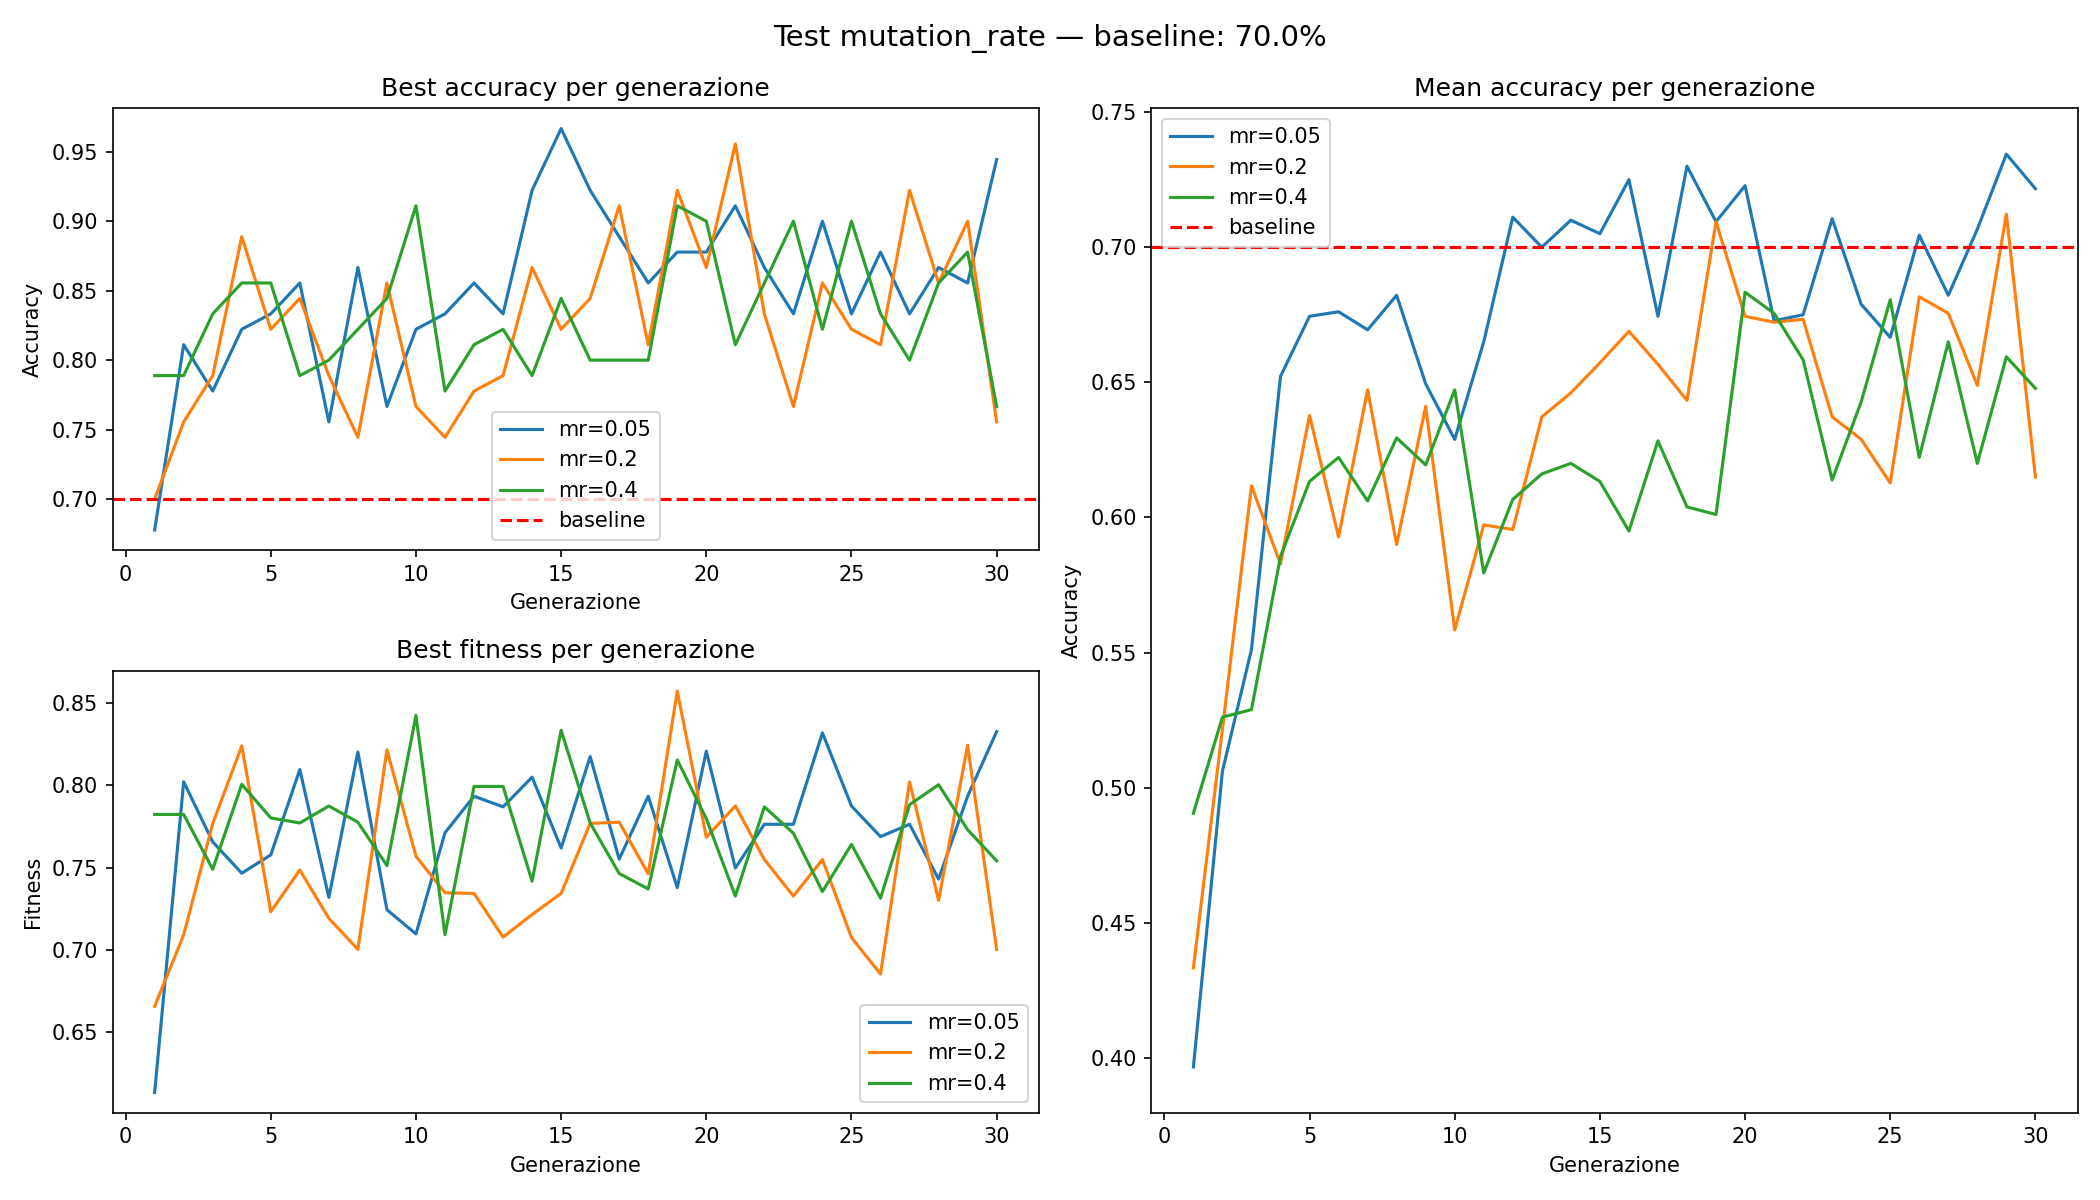
\includegraphics[width=\textwidth]{./img/test_mutation_rate.png}
    \caption{Evoluzione della fitness e accuracy al variare del mutation rate.}
    \label{fig:mutation_rate}
\end{figure}

\noindent\textbf{Osservazioni principali:}

\textbf{Tutte le run battono la baseline} con miglioramenti tra +21\% e +24\%.
Questo valida l'approccio indipendentemente dal mutation rate scelto.

\textbf{Mutation rate basso (0.05)} trova la migliore accuracy (94.44\%) ma
genera architetture più complesse (2235 parametri), risultando nella fitness
più bassa (83.27) per via della penalità. Con poca mutazione il GA si affida
al solo crossover, che tende a preservare reti grandi.

\textbf{Mutation rate medio (0.20)} ottiene la fitness più alta (85.73) con
architettura più snella (1298 parametri): miglior compromesso tra accuratezza
e complessità.

\textbf{Mutation rate alto (0.40)} introduce troppo rumore, rendendo difficile
accumulare miglioramenti. La curva della mean accuracy è la più bassa e
rumorosa lungo tutta la run.

\textit{Valore ottimale: \textbf{mutation\_rate = 0.2}}

% ────────────────────────────────────────────────────────────
\subsection{Test 2 — Lambda (Penalità di Complessità)}
% ────────────────────────────────────────────────────────────

\begin{center}
\begin{tabular}{lcccc}
    \toprule
    \rowcolor{headerblue}
    \textcolor{white}{\textbf{lambda}} &
    \textcolor{white}{\textbf{best\_accuracy}} &
    \textcolor{white}{\textbf{best\_fitness}} &
    \textcolor{white}{\textbf{n\_layer}} &
    \textcolor{white}{\textbf{n\_params}} \\
    \midrule
    0.0    & 98.89\% & 98.89 & 7 & 5447 \\
    \rowcolor{rowgray}
    0.00005 & 88.89\% & 87.83 & 1 & 211  \\
    0.0002  & 84.44\% & 80.06 & 1 & 219  \\
    \rowcolor{rowgray}
    Baseline & 60.00\% & ---  & 2 & ---  \\
    \bottomrule
\end{tabular}
\end{center}

\begin{figure}[H]
    \centering
    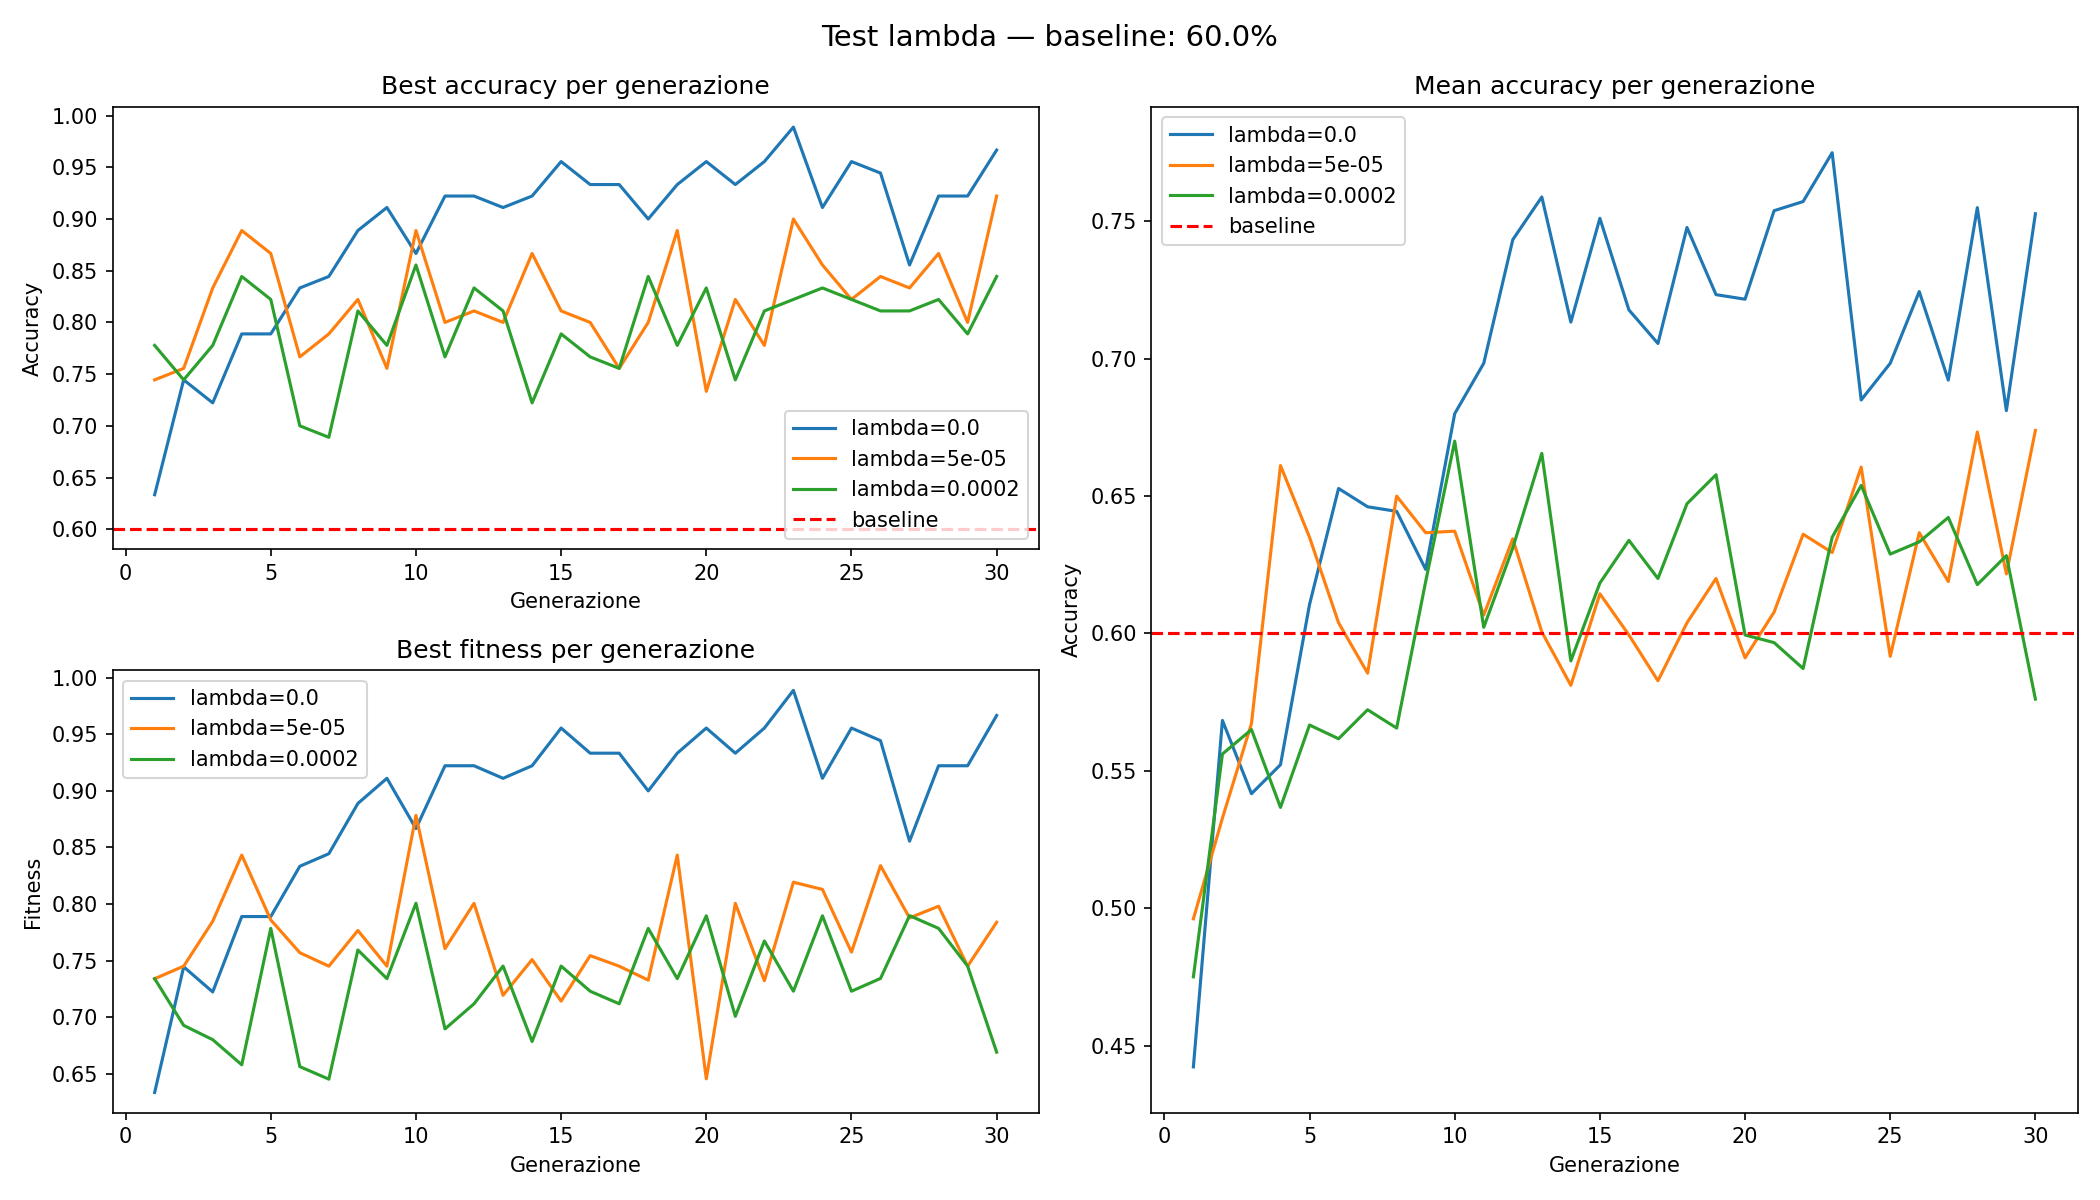
\includegraphics[width=\textwidth]{img/test_lambda.png}
    \caption{Evoluzione della fitness e accuracy al variare di lambda.}
    \label{fig:lambda}
\end{figure}

\noindent\textbf{Osservazioni principali:}

\textbf{Con $\lambda=0$} fitness e accuracy coincidono (nessuna penalità) e
il GA trova 7 layer con 5447 parametri: massimizza solo l'accuracy senza
nessun costo per la complessità. Condizioni ideali per overfitting su dataset
più complessi.

\textbf{Con $\lambda=0.00005$} la complessità si riduce del 96\%: da 5447 a
211 parametri. Anche una penalità piccola è sufficiente perché su 5447
parametri vale $0.00005 \times 5447 = 0.27$ (27 punti di accuracy sottratti).

\textbf{Con $\lambda=0.0002$} il GA trova architetture troppo semplici
sacrificando troppa accuracy. Lambda è troppo aggressivo.

\textit{Valore ottimale: \textbf{lambda = 0.00005}}

% ────────────────────────────────────────────────────────────
\subsection{Test 3 — Numero di Epoche}
% ────────────────────────────────────────────────────────────

\begin{center}
\begin{tabular}{lcccc}
    \toprule
    \rowcolor{headerblue}
    \textcolor{white}{\textbf{epochs}} &
    \textcolor{white}{\textbf{best\_accuracy}} &
    \textcolor{white}{\textbf{best\_fitness}} &
    \textcolor{white}{\textbf{n\_layer}} &
    \textcolor{white}{\textbf{n\_params}} \\
    \midrule
    50       & 75.56\% & 74.30 & 1 & 251 \\
    \rowcolor{rowgray}
    150      & 90.00\% & 88.75 & 1 & 251 \\
    300      & 92.22\% & 91.13 & 1 & 219 \\
    \rowcolor{rowgray}
    Baseline & 70.00\% & ---   & 2 & --- \\
    \bottomrule
\end{tabular}
\end{center}

\begin{figure}[H]
    \centering
    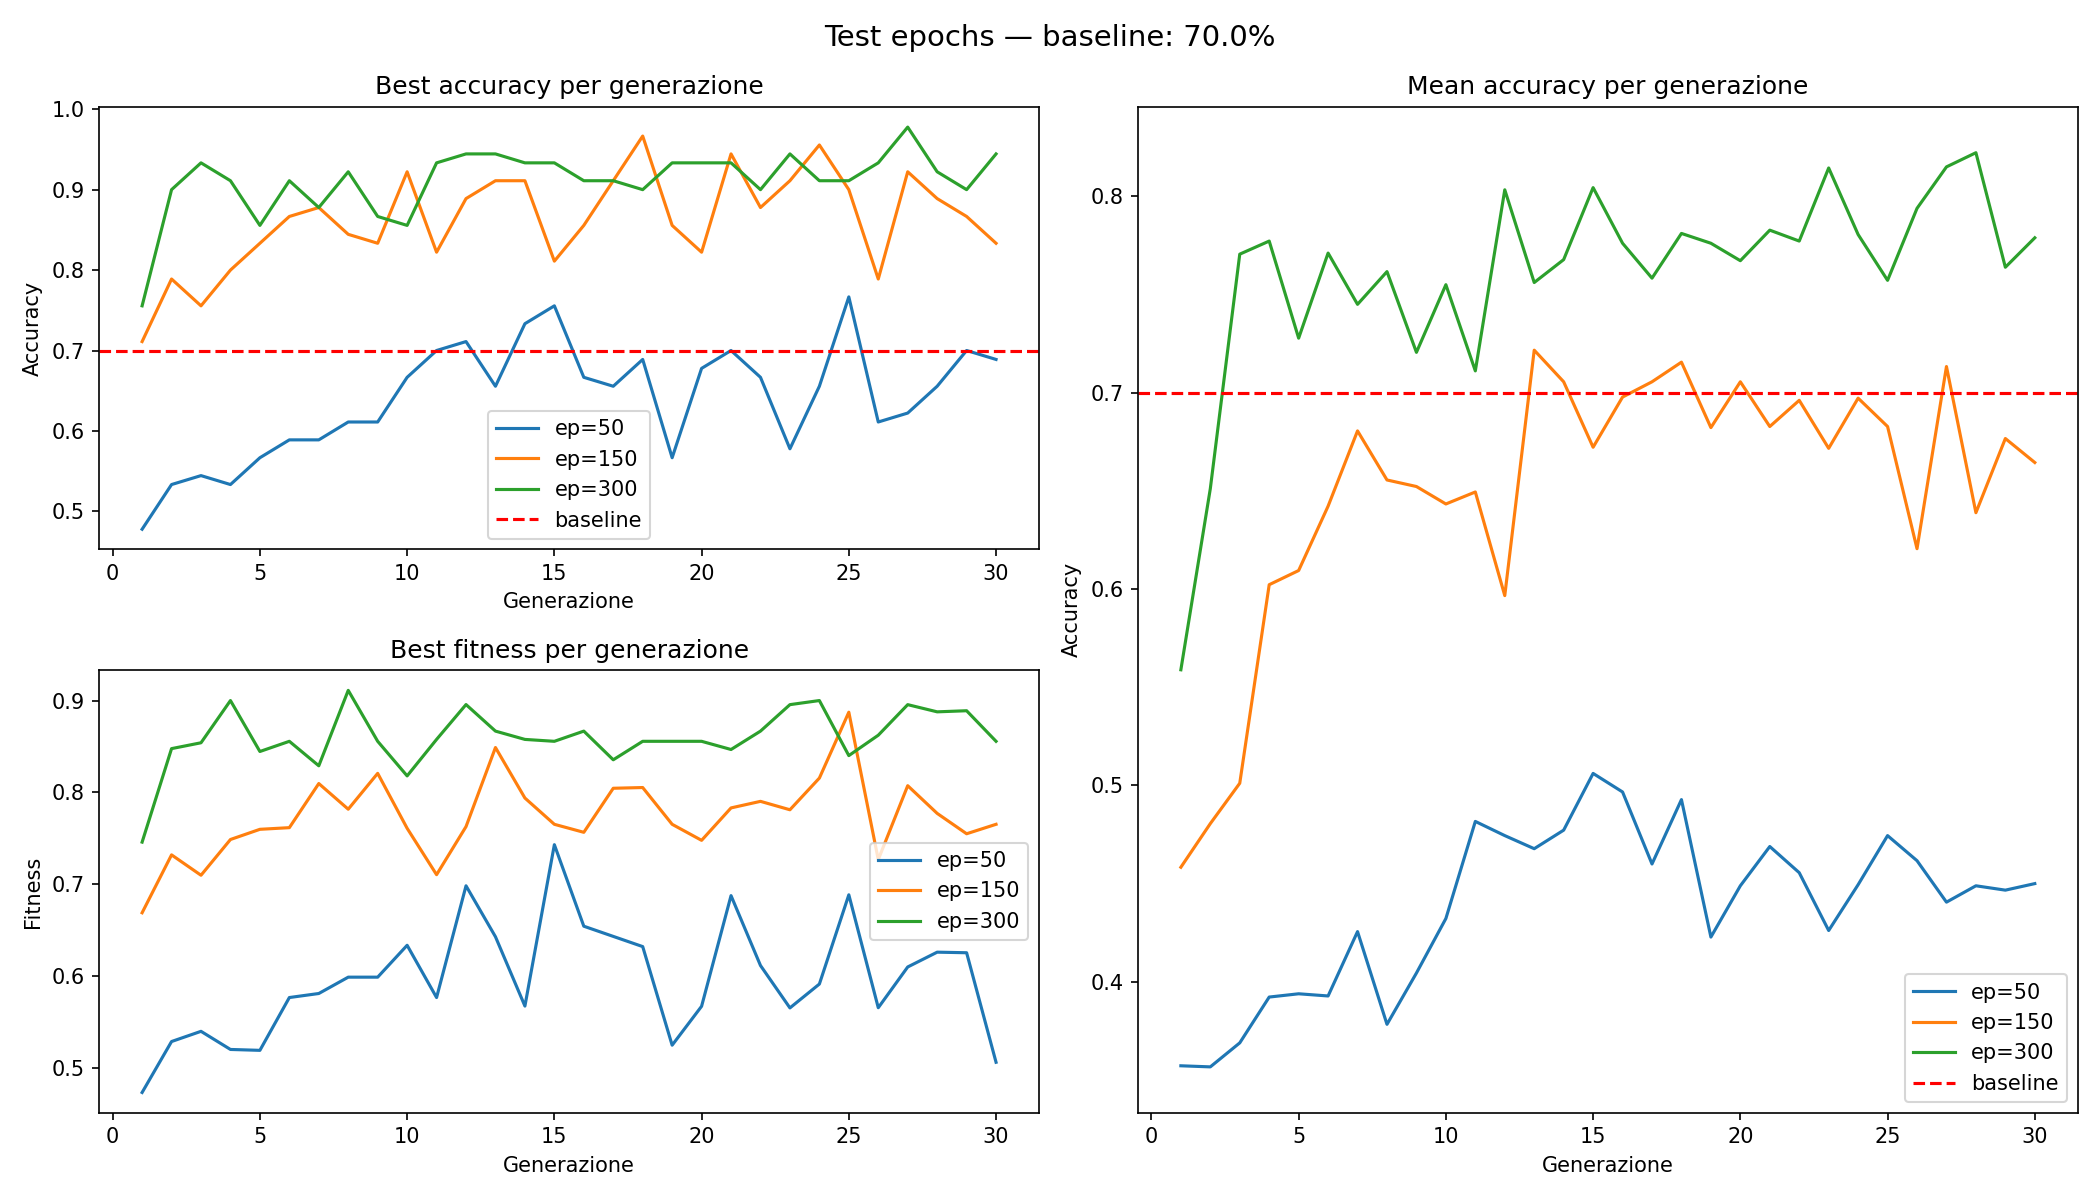
\includegraphics[width=\textwidth]{img/test_epochs.png}
    \caption{Evoluzione della fitness e accuracy al variare del numero di epoche.}
    \label{fig:epochs}
\end{figure}

\noindent\textbf{Osservazioni principali:}

\textbf{Con 50 epoche} la backpropagation non converge: i pesi restano quasi
casuali e la fitness non è informativa. Il GA non riesce a distinguere
architetture buone da cattive e non evolve efficacemente.

\textbf{Da 150 a 300 epoche} il miglioramento è solo +2.22\% a fronte di un
raddoppio del tempo totale di esecuzione ($20 \times 3 \times 300 \times 30
= 540.000$ training). Caso classico di \textbf{rendimenti decrescenti}.

\textit{Valore ottimale: \textbf{epochs = 150}}

% ────────────────────────────────────────────────────────────
\subsection{Test 4 — Learning Rate}
% ────────────────────────────────────────────────────────────

\begin{center}
\begin{tabular}{lccccc}
    \toprule
    \rowcolor{headerblue}
    \textcolor{white}{\textbf{learning\_rate}} &
    \textcolor{white}{\textbf{best\_accuracy}} &
    \textcolor{white}{\textbf{best\_fitness}} &
    \textcolor{white}{\textbf{n\_layer}} &
    \textcolor{white}{\textbf{n\_params}} \\
    \midrule
    0.001    & 60.00\% & 59.35 & 1 & 131 \\
    \rowcolor{rowgray}
    0.010    & 90.00\% & 85.36 & 2 & 928 \\
    0.050    & 96.67\% & 95.65 & 1 & 203 \\
    \rowcolor{rowgray}
    Baseline & 70.00\% & ---   & 2 & --- \\
    \bottomrule
\end{tabular}
\end{center}

\begin{figure}[H]
    \centering
    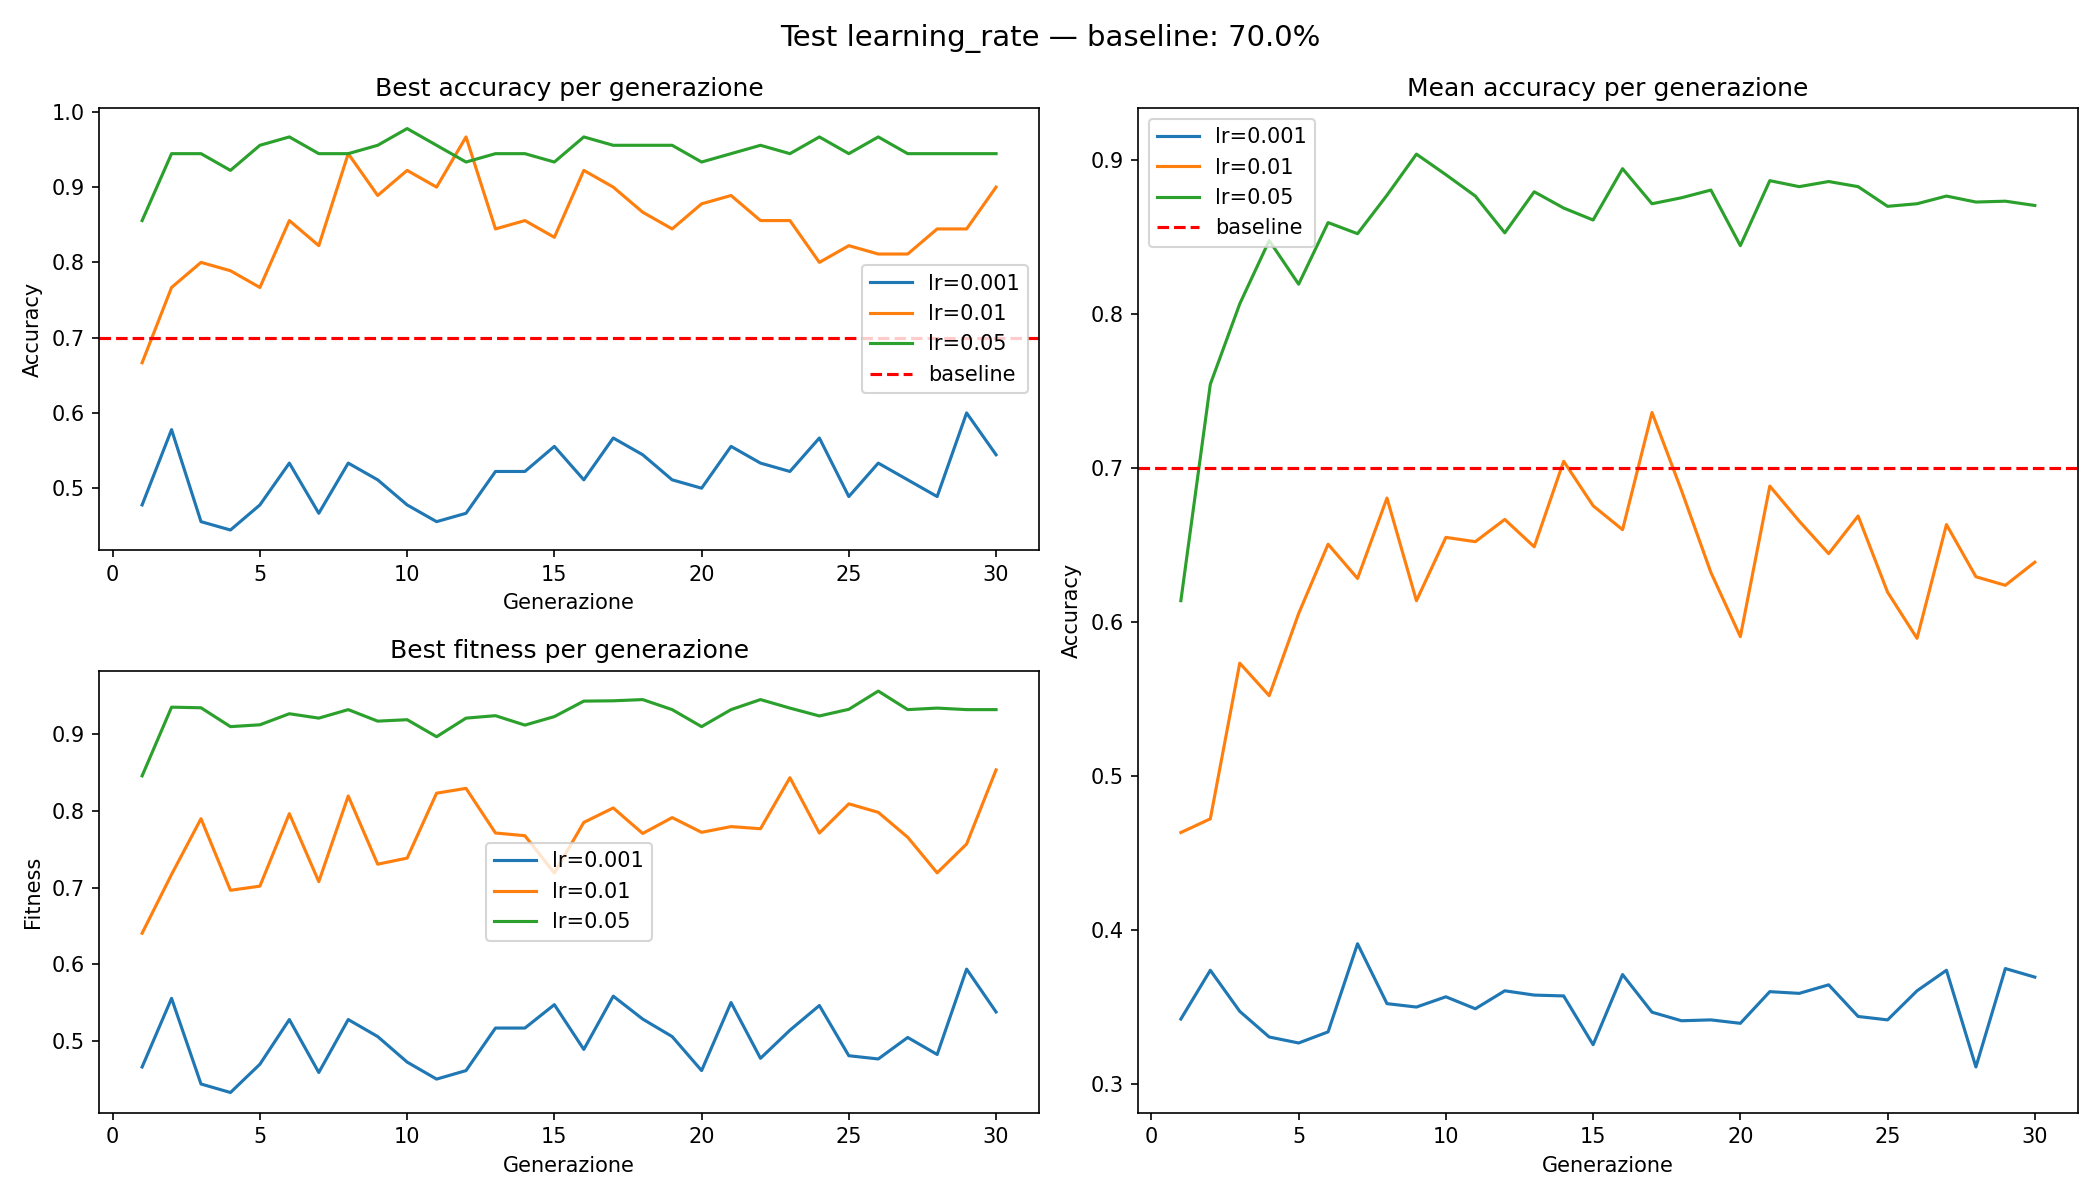
\includegraphics[width=\textwidth]{img/test_learning_rate.png}
    \caption{Evoluzione della fitness e accuracy al variare del learning rate.}
    \label{fig:lr}
\end{figure}

\noindent\textbf{Osservazioni principali:}

\textbf{Il learning rate è il parametro più critico} dell'intero sistema:
la differenza tra caso peggiore e migliore è di 36.67 punti percentuali
di accuracy, il range più ampio tra tutti i test.

\textbf{Con lr=0.001} il GA non supera la baseline: la rete non converge in
150 epoche, la fitness è rumore casuale e il GA non può evolvere.

\textbf{Con lr=0.05} si ottiene il miglior risultato in assoluto: 96.67\%
con 1 solo layer e 203 parametri.

\textbf{Rischio di divergenza}: lr troppo alto può causare oscillazioni su
problemi più complessi --- i passi di aggiornamento sono così grandi che i
pesi ``saltano'' oltre il minimo della funzione di errore.

\textbf{Parallelismo con le epoche}: learning rate e numero di epoche sono
parametri complementari. Entrambi controllano la convergenza:
\[
    \text{convergenza} = f(\text{lr},\; \text{epochs})
\]
Un lr basso può essere compensato da più epoche, ma al costo del tempo.

\textit{Valore ottimale: \textbf{learning\_rate = 0.05}}

\newpage

% ════════════════════════════════════════════════════════════
\section{Discussione e Conclusioni}
% ════════════════════════════════════════════════════════════

% ────────────────────────────────────────────────────────────
\subsection{Analisi Complessiva}
% ────────────────────────────────────────────────────────────

Il GA supera la baseline in quasi tutte le configurazioni testate. Il risultato
migliore in assoluto --- 96.67\% di accuracy con lr=0.05 --- è
significativamente superiore alla baseline del 70\%. Il GA tende a trovare
architetture con 1 solo hidden layer quando la penalità è attiva, confermando
che Iris è linearmente quasi separabile e non richiede architetture profonde.

La tabella seguente riassume i valori ottimali identificati:

\begin{center}
\begin{tabular}{lll}
    \toprule
    \rowcolor{headerblue}
    \textcolor{white}{\textbf{Parametro}} &
    \textcolor{white}{\textbf{Valore ottimale}} &
    \textcolor{white}{\textbf{Motivazione}} \\
    \midrule
    mutation\_rate & 0.20    & Miglior compromesso esplorazione/sfruttamento \\
    \rowcolor{rowgray}
    lambda\_       & 0.00005 & Riduce complessità senza sacrificare accuracy  \\
    epochs         & 150     & Convergenza affidabile, tempo accettabile      \\
    \rowcolor{rowgray}
    learning\_rate & 0.05    & Convergenza rapida in 150 epoche               \\
    \bottomrule
\end{tabular}
\end{center}

% ────────────────────────────────────────────────────────────
\subsection{Limiti del Progetto}
% ────────────────────────────────────────────────────────────

\begin{itemize}
    \item \textbf{Generalizzabilità}: le architetture ottimali trovate sono
          specifiche per Iris. Su dataset più complessi il GA richiederebbe
          più generazioni e popolazione più grande.
    \item \textbf{Variabilità}: i risultati variano tra run diverse a causa
          della casualità. Per risultati affidabili servirebbero multiple run
          con media e deviazione standard.
    \item \textbf{Ottimizzatore}: la backpropagation usa SGD puro senza
          ottimizzatori moderni (Adam, RMSprop) che garantirebbero convergenza
          più rapida e stabile.
    \item \textbf{Derivata Softmax}: l'approssimazione diagonale del Jacobiano
          potrebbe essere limitante su problemi più complessi.
\end{itemize}

% ────────────────────────────────────────────────────────────
\subsection{Sviluppi Futuri}
% ────────────────────────────────────────────────────────────

\begin{itemize}
    \item Validazione su dataset più complessi (es. MNIST, Wine Quality)
    \item Implementazione del Jacobiano completo per la Softmax
    \item Aggiunta di Dropout per ridurre il rischio di overfitting
    \item Implementazione di Early Stopping nella valutazione della fitness
    \item Implementazione di Adam come ottimizzatore alternativo a SGD
    \item Esposizione di K come parametro configurabile del costruttore
\end{itemize}

\newpage

% ════════════════════════════════════════════════════════════
\appendix
\section{Glossario dei Termini Chiave}
% ════════════════════════════════════════════════════════════

\begin{description}
    \item[Accuratezza (Accuracy)] Percentuale di predizioni corrette sul
        validation set. Valore tra 0 e 1.

    \item[Backpropagation] Algoritmo per calcolare il gradiente della funzione
        di loss rispetto ai pesi della rete, propagando l'errore all'indietro
        layer per layer tramite la regola della catena.

    \item[Baseline] Rete con architettura fissa $[(8,\text{relu}),(8,\text{relu})]$
        addestrata con backpropagation classica, usata come punto di riferimento
        per valutare i risultati del GA.

    \item[Classificazione] Problema in cui l'output è una categoria discreta.
        Contrapposto alla regressione (output continuo).

    \item[Cromosoma] Rappresentazione di una soluzione candidata nel GA:
        lista di tuple \texttt{(n\_neuroni, funzione\_attivazione)}.

    \item[Crossover] Operatore genetico che combina due genitori per generare
        un figlio scambiando parti dei cromosomi.

    \item[Data leakage] Uso di informazioni del validation set durante il
        preprocessing o il training, che porta a stime ottimistiche delle prestazioni.

    \item[Elitismo] Tecnica che copia il miglior individuo nella nuova
        popolazione, garantendo che la qualità non peggiori tra generazioni.

    \item[Fitness] Misura della qualità di un individuo nel GA:
        $\text{fitness} = \text{accuracy} - \lambda \cdot N_{\text{params}}$.

    \item[Gradient descent] Algoritmo di ottimizzazione che aggiorna i
        parametri nella direzione opposta al gradiente della funzione di loss.

    \item[Learning rate ($\eta$)] Iperparametro che controlla la dimensione
        del passo di aggiornamento dei pesi durante la backpropagation.

    \item[Mutazione] Operatore genetico che introduce variazioni casuali nel
        cromosoma per mantenere diversità nella popolazione.

    \item[NAS (Neural Architecture Search)] Campo di ricerca che studia
        l'automazione della progettazione di architetture di reti neurali.

    \item[One-hot encoding] Rappresentazione delle etichette come vettori
        binari con un solo 1 nella posizione corrispondente alla classe.

    \item[Overfitting] Fenomeno per cui il modello memorizza i dati di
        training e non generalizza su dati nuovi.

    \item[Penalità di complessità] Termine $\lambda \cdot N_{\text{params}}$
        sottratto dalla fitness per favorire architetture semplici.

    \item[Pressione selettiva] Intensità con cui gli individui migliori
        vengono preferiti nella riproduzione.

    \item[Rendimenti decrescenti] Fenomeno per cui ogni unità aggiuntiva
        di una risorsa contribuisce sempre meno al miglioramento.

    \item[Selezione a torneo] Metodo che estrae K individui casuali e sceglie
        il migliore tra loro come genitore.

    \item[Softmax] Funzione di attivazione che normalizza un vettore in una
        distribuzione di probabilità. Usata solo sull'output layer per
        classificazione multi-classe.

    \item[StandardScaler] Trasformazione che porta ogni feature a media 0 e
        deviazione standard 1.

    \item[Validation set] Porzione del dataset non usata durante il training,
        per valutare le prestazioni su dati mai visti.

    \item[Vanishing gradient] Problema per cui i gradienti diventano
        estremamente piccoli nei \emph{layer iniziali} della rete durante
        la backpropagation, rallentando o impedendo l'apprendimento di
        quei layer (tipico di Sigmoid su reti profonde, dove la derivata
        satura verso 0).
\end{description}

% ════════════════════════════════════════════════════════════
\end{document}
% ════════════════════════════════════════════════════════════